\section{Työn suunnittelu} \label{suunnittelu}

Työssä luodaan sovellus, jolla on mahdollista laskea ohjelmakoodissa määriteltyjä ongelmia geneettisen algoritmin avulla.
Ongelmaa varten tulee määritellä funktio kelvollisuusarvon laskemista varten, sekä siinä esiintyvät muuttujat.
Lisäksi voidaan määrätä geneettinen algoritmi käyttämään jotain ennalta luotua valintaprosessia, jolla valitaan kunkin syklin aikana
populaation jäsenet, jotka siirtävät informaatiota seuraavaan populaatioon.

Ennen sovelluksen kehittämistä valittiin yhtälöt \ref{eq:xyz_graph} ja \ref{eq:sum}, jolla geneettisen algoritmin
aikana luotujen populaatioiden sopivuutta olisi helppo tarkastella. Yhtälössä \ref{eq:xyz_graph} voidaan visualisoida
populaatioiden kehitystä graafisesti kuvaajalla \ref{fig:xyz_graph}. Yhtälön \ref{eq:sum} teoreettinen suurin ja pienin
voidaan helposti johtaa, kun on määritelty siinä käytettävien muuttujien suurimmat ja pienimmät mahdolliset arvot. Esitetyistä yhtälöistä
luodaan maksimointiongelmat, jotka voidaan suorittaa ohjelmasta.

\begin{equation}
	\label{eq:xyz_graph}
	f(x,y) = y \sin{ \left( \sqrt {x^2 + y^2} \right) } + x \left( sign(y) \right)
\end{equation}

\begin{equation}
	\label{eq:sum}
	f(\vec a) = a_1 - a_2 + a_3 - a_4 + a_5 - a_6 + a_7 - a_8 \qquad
	\{\vec a \in \mathbb R^8\}
\end{equation}

\begin{figure}[H]
	\caption{
		Yhtälössä \ref{eq:xyz_graph} esitetyn funktion kuvaaja \(xyz\)-tasossa välillä
		\((x,y,z) = ([-20, 20], [-20, 20], [-40, 40])\)
	}
	\centering
	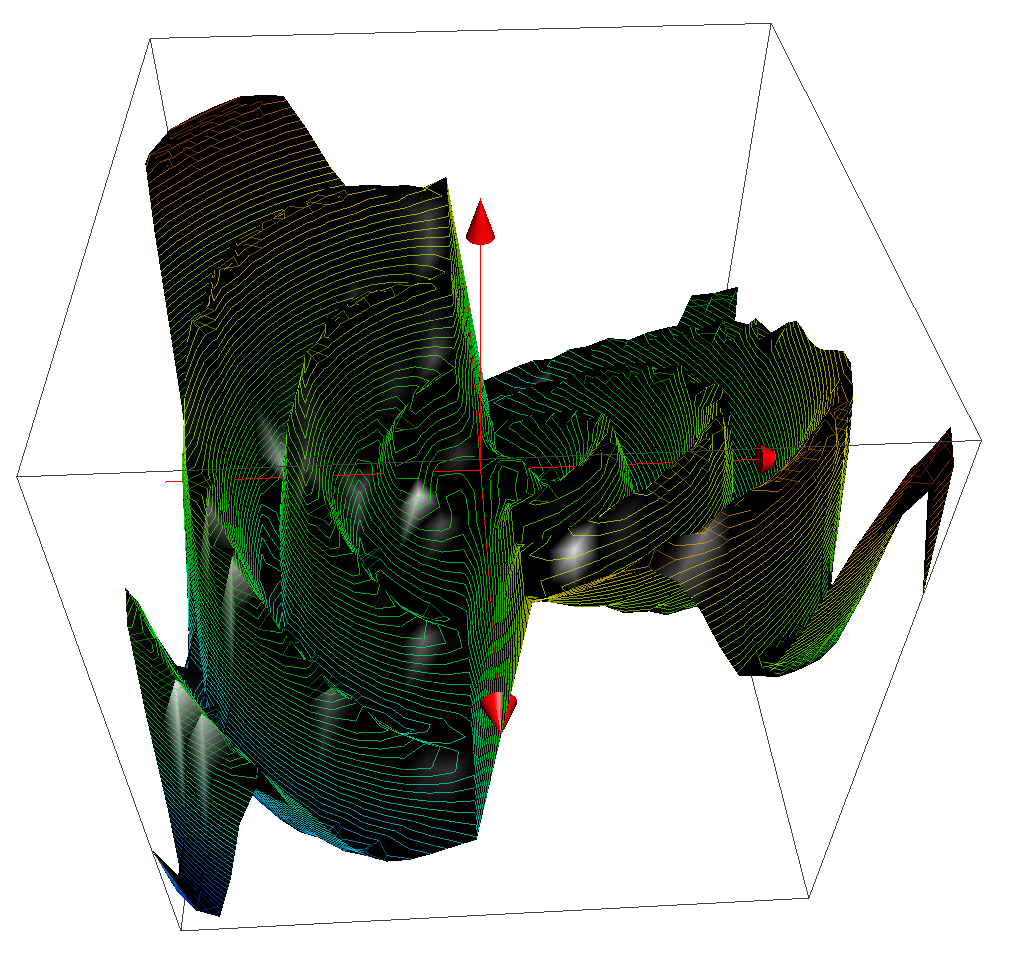
\includegraphics[width=12cm]{xyz_graph}
	\label{fig:xyz_graph}
\end{figure}

Koska tarkasteltaville muuttujille annetaan arvo niille määritetyn maksimi- ja minimiarvon väliltä, päädyttiin
genotyyppien alleelit esittämään liukulukuarvoin. Alleelit voivat saada lukuarvoja väliltä \([0, 1]\), ja kun
genotyypit käännetään fenotyypeiksi, skaalataan kunkin muuttujaan liitetyn alleelin arvon
perusteella luku muuttujan maksimi ja minimiarvon välillä. Kun fenotyypin arvot on johdettu, voidaan ne
edelleen syöttää funktioon, joka laskee alkiolle kelvollisuusarvon.

Mutaation todennäköisyys on syytä pitää matalana, sillä muutoin geneettinen algoritmi muuttuu liian satunnaiseksi.
Jos alleelien arvot olisivat muodoltaan binäärilukuja, mutaatio voitaisiin toteuttaa siten, että mutatoituvissa
alleeleissa arvo 0 muutetaisiin arvoon 1. Koska työssä olevien alleelien arvot ovat liukulukuja väliltä \([0,1]\),
toteutetaan mutaatio siten, että mutatoitavaan alleeliin lisätään satunnainen arvo joka voi olla myös negatiivinen.
Jotta mutaatiosta saadaan hienovaraisempaa, satunnainen arvo lasketaan siten,
että mitä lähempänä nollaa arvo on, sen todennäköisempää sen valinta on.
Työssä kaikille genotyypin alleeleille annetaan mahdollisuus mutaatioon,
joten yhden syklin aikana alkioon voi tapahtua teoriassa yhtä monta mutaatiota, kun siinä on alleeleja.

Sovellus toteutetaan oliopohjaisena Scala -ohjelmointikieltä käyttäen. Kutakin ongelmaa varten luodaan valvoja (\textit{Overseer})
luokan olio, joka vastaa geneettisen algoritmin suorittamisesta ja sen parametrien hallinnasta.
Ohjelmaan ei tule graafista käyttöliittyymää ja sitä ohjataan komentoriviltä.
Ohjelman käyttäjän tulee voida valita ratkaistava ongelma, populaation koko,
mutaation ja risteytyksen todennäköisyys, sekä pystyä hallinnoimaan ongelmaa varten määriteltyjen muuttujien arvoja.
